\documentclass[logo,reportComp]{thesis}
\usepackage[cpp]{mypackage}

\title{计算机网络实验报告}
\subtitle{实验一:数据表示实验}
\school{数据科学与计算机学院}
\author{陈鸿峥}
\classname{17大数据与人工智能}
\stunum{17341015}
\headercontext{计算机网络实验报告}

\begin{document}

\maketitle

\section{实验目的}
掌握结构数据的保存和读取方法。

\section{实验说明}
\begin{itemize}
	\item 把源程序和可执行文件放在相应的上交源码目录中
	\item 截屏用按键(Ctrl+Alt+PrintScreen)截取当前窗口
\end{itemize}

\section{参考资料}
\begin{itemize}
	\item C语言函数分类:\url{http://msdn.microsoft.com/zh-cn/library/2aza74he(v=vs.110).aspx}
	\item C语言字符串函数:\url{http://msdn.microsoft.com/zh-cn/library/f0151s4x(v=vs.110).aspx}
\end{itemize}

\section{实验环境}
本机为Ubuntu 18.04(LTS) + gcc 7.3.0

\section{实验内容}
\subsection{结构数据保存和读出}
\subsubsection{实验要求}
循环输入员工(\verb'Person')的信息,每输入一个员工的信息,立即写入文件(\verb'Persons.txt'),直到输入的姓名为空时跳出循环。
然后读出该文件,显示每个\verb'Person'的信息。

\verb'Person'的信息表示:
\begin{lstlisting}
struct Person {
   char username[USER_NAME_LEN];
   int level;
   char email[EMAIL_LEN];
   DWORD sendtime;
   time_t regtime;
}; 
\end{lstlisting}

\subsubsection{运行结果}
控制行运行结果如下,并在当前文件夹中产生文件\verb'Persons.txt'。
\begin{figure}[H]
\centering
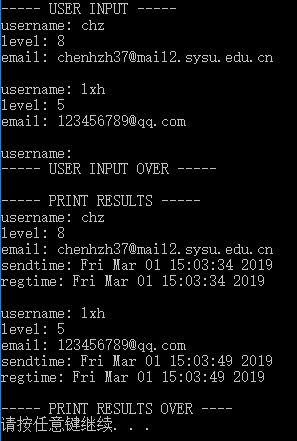
\includegraphics[width=0.4\linewidth]{fig/person.PNG}
\end{figure}

\subsubsection{源代码}
\begin{lstlisting}
#include <stdio.h>
#include <stdlib.h>
#include <string.h>
#include <time.h>

#define BUF_LEN 100
#define USER_NAME_LEN 20
#define EMAIL_LEN 80
#define TIME_BUF_LEN 30
#define MAX_PEOPLE 100

typedef unsigned long DWORD;

typedef struct Person {
    char username[USER_NAME_LEN];
    int level;
    char email[EMAIL_LEN];
    DWORD sendtime;
    time_t regtime;
} Person;

int main()
{
	Person people[MAX_PEOPLE];
	FILE* pfile;
	int i;
	// Input
	pfile = fopen("./Persons.txt","wb");
	printf("----- USER INPUT -----\n");
	for (i = 0; i < MAX_PEOPLE; ++i){
		fflush(stdin);
		char name[USER_NAME_LEN];
		printf("username: ");
		gets(name);
		if (name[0] == '\0')
			break;
		strcpy(people[i].username,name);
		fprintf(pfile, "%s\n", name);

		int l;
		printf("level: ");
		scanf("%d",&l);
		people[i].level = l;
		fprintf(pfile, "%d\n", l);

		char email[EMAIL_LEN];
		printf("email: ");
		scanf("%s",&email);
		strcpy(people[i].email,email);
		fprintf(pfile, "%s\n", email);

		time_t now; // current time
		time (&now);  // get now time
		struct tm* lt = localtime (&now);
		people[i].sendtime = (DWORD)now;
		people[i].regtime = now;
		fprintf(pfile, "%ld\n", people[i].sendtime);
		fprintf(pfile, "%ld\n", people[i].regtime);

		printf("\n");
	}
	fclose(pfile);
	printf("----- USER INPUT OVER -----\n\n");

	// Read the file
	pfile = fopen("Persons.txt","r");
	if (pfile == NULL)
		exit(EXIT_FAILURE);
	printf("----- PRINT RESULTS -----\n");
	for (i = 0; i < MAX_PEOPLE; ++i){
		char name[USER_NAME_LEN];
		if (fscanf(pfile,"%s",name) != 1)
			break;
		printf("username: %s\n", name);

		int l;
		fscanf(pfile,"%d",&l);
		printf("level: %d\n", l);

		char email[EMAIL_LEN];
		fscanf(pfile,"%s",email);
		printf("email: %s\n",email);

		char buf[TIME_BUF_LEN];
		time_t sendtime;
		fscanf(pfile,"%ld",&sendtime);
		struct tm* lt = localtime (&sendtime);
		// Www Mmm dd hh:mm:ss yyyy\n
		strftime(buf,TIME_BUF_LEN,"%a %b %d %H:%m:%S %Y",lt);
		printf("sendtime: %s\n", buf);
		
		time_t regtime;
		fscanf(pfile,"%ld",&regtime);
		lt = localtime (&regtime);
		strftime(buf,TIME_BUF_LEN,"%a %b %d %H:%m:%S %Y",lt);
		printf("regtime: %s\n", buf);

		printf("\n");
	}
	printf("----- PRINT RESULTS OVER ----\n");
	fclose(pfile);
	return 0;
}
\end{lstlisting}

\subsection{多文件合并保存和读出}
\subsubsection{实验要求}
循环输入多个文件名(不超过200MB,可以自己确定),每输入一个,就把该文件的文件名(最多300字节)、文件大小(long)和文件内容写入文件\verb'FileSet.pak'中,输入文件名为空时跳出循环。
然后读\verb'FileSet.pak',每读出一个文件就把它原来的文件名加上一个序号保存起来。

注意:合并时可以先取得文件大小,然后边读边写。

\subsubsection{运行结果}
运行程序控制行结果如下
\begin{figure}[H]
\centering
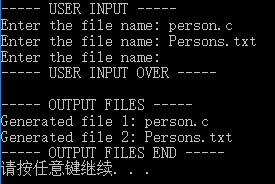
\includegraphics[width=0.4\linewidth]{fig/file-copy.PNG}
\end{figure}

文件生成展示如下,见最后一列可见生成文件与原文件大小相同。
\begin{figure}[H]
\centering
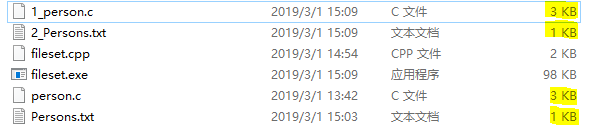
\includegraphics[width=0.7\linewidth]{fig/file-copy-res.PNG}
\end{figure}

\subsubsection{与同学互测并截屏运行结果}
把保存的文件给同学,看他是否可以可以取出其中文件,同样可以测试是否可以读出并保存同学的文件。
注意结构要相同。

从下面的结果可以看出两个文件的内容相同。(左侧为同学发给我的\verb'1_test.txt'文件,右侧为生成的\verb'1_1_test.txt'文件。)
\begin{figure}[H]
\centering
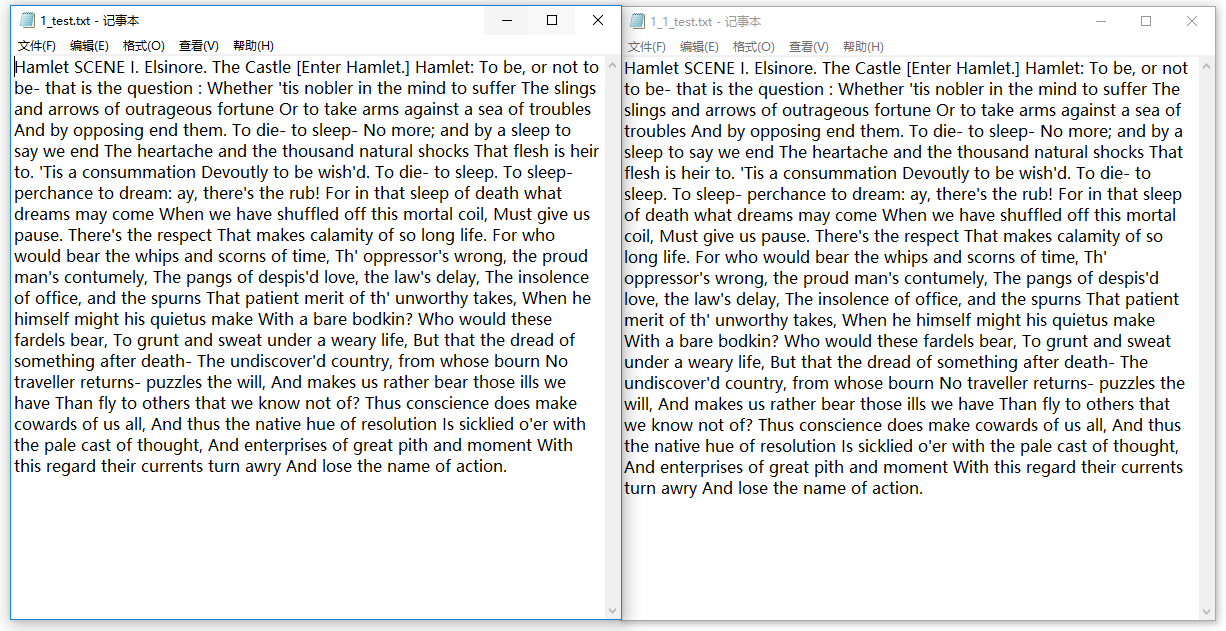
\includegraphics[width=0.8\linewidth]{fig/test.PNG}
\end{figure}

\subsubsection{源代码}
\begin{lstlisting}
#include <iostream>
#include <fstream>
#include <cstdlib>
#include <string>
using namespace std;

#define FILE_NAME "FileSet.pak"

int main()
{
	ofstream output(FILE_NAME);
	cout << "----- USER INPUT -----" << endl;
	while (true){
		cout << "Enter the file name: ";
		string filename;
		getline(cin,filename);
		if (filename == "")
			break;

		FILE *p_file = fopen(filename.c_str(),"rb");
		fseek(p_file,0,SEEK_END);
		long size = ftell(p_file);
		fclose(p_file);

		output << filename << endl;
		output << size << endl;
		// output << "##### FILE BEGIN #####" << endl;
		ifstream input(filename);
		string str;
		while (getline(input,str))
			output << str << endl;
		// output << "##### FILE OVER #####" << endl;
	}
	cout << "----- USER INPUT OVER -----\n" << endl;

	// read in file
	ifstream input(FILE_NAME);
	cout << "----- OUTPUT FILES -----" << endl;
	for (int i = 1; true ; ++i){
		string str, filename;
		if (!getline(input,filename))
			break;
		getline(input,str); // size
		long exp_size = stol(str);
		// getline(input,str); // ##### FILE BEGIN #####
		ofstream output(to_string(i)+"_"+filename);
		while (getline(input,str)){
			// if (str.find("#####") != string::npos){ // ##### FILE OVER #####
			output << str << endl;
			FILE *p_file = fopen((to_string(i)+"_"+filename).c_str(),"rb");
			fseek(p_file,0,SEEK_END);
			long size = ftell(p_file);
			fclose(p_file);
			if (size >= exp_size){
				break;
			}
		}
		cout << "Generated file " << i << ": " << filename << endl;
	}
	cout << "----- OUTPUT FILES END -----" << endl;
	return 0;
}
\end{lstlisting}

\section{完成情况}
\begin{itemize}
	\item 是否完成以下步骤?(\cmark完成\quad\xmark未做)\\
	1. [\cmark]\qquad 2. [\cmark]
	\item 是否与同学进行了互测? [\cmark] \\
	互评同学学号姓名:17341111刘学海
\end{itemize}

\section{实验体会}
% 写出实验过程中遇到的问题,解决方法和自己的思考;并简述实验体会(如果有的话)。
虽然该实验比较简单,但还是遇到了比较多的问题。

因为平常经常写C++程序,C的文件流操作很多都已经忘了,因而\textbf{第一个实验}对于\textbf{字符串的操作处理}并不得心应手。
查了很多C的字符串函数,才顺利完成任务。

对于\textbf{第二个实验},最大的难点则是判断每一个文件到\textbf{哪一行终止},因为在\verb'FileSet.pak'中,所有文件都存储在一起,又没有行号标识就很难分开。
最后采取了效率比较低的方法,即每写完输出文件的一行之后,就立即判断这时输出文件的大小,如果仍然小于给定的大小,则继续读该文件,否则属于下一文件。

总的来说,基础C的字符串操作还是应熟悉,毕竟对于比较底层的操作C还是比C++用得多(如操作系统)。

\end{document}
% 【交实验报告】
% 每位同学单独完成本实验内容并填写实验报告。
%     交作业地点:http://172.18.187.11/netdisk/default.aspx?vm=17net 
% 编程实验 
% 截止日期:2019年3月9日23:00(周六)。
% 上传文件:学号_姓名_数据表示实验报告.doc
% 学号_姓名_数据表示实验源码.rar (源程序和可执行程序)